\documentclass[11pt, a4paper]{article}

% --- PACOTES PRINCIPAIS (os do template fornecido) ---
\usepackage[utf8]{inputenc}
\usepackage[T1]{fontenc}
\usepackage{geometry}
\geometry{a4paper, top=2.5cm, bottom=2.5cm, left=2.0cm, right=2.0cm}
\usepackage{amsmath, amssymb, amsfonts}
\usepackage{booktabs}
\usepackage{tabularx}
\usepackage{graphicx}
\usepackage{xcolor}
\usepackage{enumitem}
\usepackage{tcolorbox}
\usepackage{fancyhdr}
\usepackage[colorlinks=true, linkcolor=ufopred, citecolor=deepnavy, urlcolor=ufopred]{hyperref}

% Idioma: português do Brasil (nomes "Tabela"/"Figura" e hifenização).
% Se o pacote de idioma não estiver instalado, só os nomes são ajustados.
\IfFileExists{brazilian.ldf}{\usepackage[brazilian]{babel}}{%
  \AtBeginDocument{\renewcommand{\tablename}{Tabela}\renewcommand{\figurename}{Figura}}}

% --- CORES INSTITUCIONAIS UFOP ---
\definecolor{ufopred}{RGB}{140, 29, 36}
\definecolor{deepnavy}{RGB}{20, 35, 60}
\definecolor{lightgray}{RGB}{245, 247, 250}
\definecolor{darkslate}{RGB}{30, 40, 50}

% --- CONFIGURAÇÃO DE CABEÇALHO E RODAPÉ ---
\pagestyle{fancy}
\fancyhf{}
\setlength{\headheight}{14pt}
\rhead{\textcolor{darkslate}{\small \textbf{Plataforma CCO/UFOP} --- Artigo Científico}}
\lhead{\textcolor{darkslate}{\small Computação Gráfica --- TP1 (BCC327)}}
\cfoot{\thepage}

\tcbuselibrary{skins, breakable}

% --- MACROS DO TRABALHO ---
% valor que depende dos modelos VTK (aparece em vermelho; preencher antes de entregar)
\newcommand{\preencher}[1]{\textcolor{red}{\textbf{[#1]}}}

% figura que só existe depois de rodar o programa com um VTK: se o arquivo
% ainda não estiver em figures/, aparece uma caixa vermelha no lugar.
\newcommand{\figarq}[4]{% arquivo, largura, legenda, rótulo
  \begin{figure}[htbp]\centering
    \IfFileExists{figures/#1.png}
      {\includegraphics[width=#2\linewidth]{figures/#1.png}}
      {\fbox{\parbox{0.8\linewidth}{\centering\color{red}\vspace{1.5em}
        Gerar \texttt{\detokenize{figures/#1.png}}\vspace{1.5em}}}}
    \caption{#3}\label{#4}
  \end{figure}}

\newcommand{\fig}[4]{% figura sempre presente
  \begin{figure}[htbp]\centering
    \includegraphics[width=#2\linewidth]{figures/#1.png}
    \caption{#3}\label{#4}
  \end{figure}}

\newcommand{\arq}[1]{\texttt{#1}}

\begin{document}

% --- TÍTULO E AUTORES ---
\begin{center}
  {\LARGE \bfseries \textcolor{ufopred}{Visualização Geométrica, Rasterização e Recorte de Árvores Arteriais CCO}}\\[0.4cm]
  {\large \textbf{João Pedro Silva Cruz}$^{1}$, \textbf{Pedro Vítor Silva Cruz}$^{1}$}\\[0.2cm]
  {\small $^{1}$Departamento de Computação (DECOM) --- Universidade Federal de Ouro Preto (UFOP)\\[0.1cm]
  BCC327 --- Computação Gráfica --- 2026.2 --- Trabalho Prático 1\\[0.1cm]
  \texttt{\{joao.prsc@aluno.ufop.edu.br, pedro.vsc@aluno.ufop.edu.br\}}}\\[0.4cm]
\end{center}

% --- CAIXA DE RESUMO E PALAVRAS-CHAVE ---
\begin{tcolorbox}[colback=lightgray, colframe=deepnavy, arc=3pt, title=\textbf{RESUMO}, fonttitle=\bfseries]
\small
\textbf{Contexto:} Modelos de árvores arteriais geradas pelo método \emph{Constrained Constructive Optimization} (CCO) são descritos por pontos, segmentos e um raio por vaso, e servem de cena para estudar os algoritmos clássicos de Computação Gráfica.
\textbf{Objetivo:} Construir uma aplicação que leia modelos CCO em formato VTK e os visualize, transforme, rasterize e recorte, deixando explícito o que é implementação própria e o que vem de bibliotecas (trabalho prático 1 da disciplina BCC327).
\textbf{Metodologia:} Leitura e janela 3D com PyVista/VTK; matrizes de modelo, vista e projeção, Bresenham, \emph{Scanline Fill}, \emph{supersampling} e os recortes de Cohen--Sutherland, Liang--Barsky, Cyrus--Beck e Sutherland--Hodgman implementados em Python e NumPy; interface em PyQt5.
\textbf{Resultados:} Os algoritmos foram validados por autotestes aleatórios (por exemplo, 20\,000 segmentos nos quais os três recortes de segmentos coincidem; 600 polígonos no Sutherland--Hodgman) e demonstrados em exemplos numéricos; na cena de teste, o \emph{supersampling} $4\times4$ reduziu o erro quadrático médio de 2414,0 para 54,1.
\textbf{Conclusão:} A aplicação integra os sete módulos pedidos; o caso do polígono côncavo em U evidencia a limitação do Sutherland--Hodgman e o motivo de se usar o Weiler--Atherton.

\vspace{0.2cm}
\textbf{Palavras-Chave:} Computação Gráfica; Método CCO; Rasterização; Antialiasing; Recorte; VTK.
\end{tcolorbox}

\vspace{0.4cm}

% --- SEÇÃO 1: INTRODUÇÃO ---
\section{Introdução}
Modelos computacionais de árvores vasculares são usados para estudar a
geometria e a perfusão de órgãos. O método CCO constrói esses modelos
adicionando segmentos a uma árvore de modo a minimizar um custo sujeito a
restrições~\cite{schreiner1993,karch1999}. O resultado é uma estrutura
geométrica simples: pontos no plano ou no espaço, segmentos de reta que os
ligam e um atributo por vaso, o raio.

O objetivo deste trabalho não é gerar essas árvores (os modelos 2D e 3D foram
fornecidos pelo professor), e sim usá-las como cena para aplicar e comparar
os algoritmos clássicos de Computação Gráfica. Os objetivos específicos, um por
módulo do enunciado, são:
\begin{enumerate}[leftmargin=*]
  \item ler os arquivos VTK e apresentar número de pontos e segmentos, raio mínimo e
        máximo, primitivas e atributos visuais (Módulo~1);
  \item aplicar translação, rotação e escala, posicionar o observador em várias vistas e
        comparar as projeções ortográfica e perspectiva (Módulo~2);
  \item rasterizar segmentos com Bresenham (Módulo~3) e preencher polígonos por
        \emph{Scanline} (Módulo~4);
  \item comparar a imagem com e sem antialiasing (Módulo~5);
  \item recortar segmentos (Módulo~6) e polígonos (Módulo~7).
\end{enumerate}
O trabalho também documenta, de forma explícita, o que foi implementado pelo grupo
e o que veio das bibliotecas (Seção~\ref{sec:autoria}).

% --- SEÇÃO 2: TRABALHOS RELACIONADOS ---
\section{Trabalhos Relacionados}
O método CCO foi introduzido por Schreiner e Buxbaum~\cite{schreiner1993} e estendido a árvores tridimensionais por Karch et al.~\cite{karch1999}. Neste trabalho essas árvores são apenas o dado de entrada: os modelos 2D e 3D foram fornecidos pelo professor, e o método de geração não foi reimplementado. Do lado da Computação Gráfica, os algoritmos aplicados são clássicos e estão descritos em livros-texto~\cite{foley1990}; a visualização interativa usa o VTK~\cite{vtk} por meio do PyVista~\cite{pyvista}. A Tabela~\ref{tab:relacionados} resume o papel de cada referência no trabalho.

\begin{table}[htbp]
  \centering
  \small
  \caption{Referências principais e seu uso neste trabalho.}
  \label{tab:relacionados}
  \begin{tabularx}{\textwidth}{l X X}
    \toprule
    \textbf{Tópico} & \textbf{Referência} & \textbf{Uso neste trabalho} \\
    \midrule
    Geração de árvores CCO & Schreiner e Buxbaum (1993); Karch et al. (1999) & Origem dos modelos VTK 2D e 3D; método não reimplementado \\
    Rasterização de linhas & Bresenham (1965) & Implementado (8 octantes, aritmética inteira); DDA para comparação \\
    Recorte de segmentos & Cohen--Sutherland~\cite{foley1990}; Liang e Barsky (1984); Cyrus e Beck (1978) & Os três implementados e comparados \\
    Recorte de polígonos & Sutherland e Hodgman (1974); Weiler e Atherton (1977) & Sutherland--Hodgman implementado; Weiler--Atherton apenas discutido \\
    Visualização 3D & VTK; PyVista & Leitura do arquivo, janela OpenGL, tubos e antialiasing do VTK \\
    \bottomrule
  \end{tabularx}
\end{table}


%% =====================================================================
\section{Fundamentação Teórica e Metodologia}

\subsection{Árvores CCO e o arquivo VTK}
No CCO, a árvore cresce por inserção sucessiva de terminais; cada vaso é um
segmento com raio próprio~\cite{schreiner1993}. A versão 3D, usada em
\cite{karch1999}, representa a árvore no espaço. Para este trabalho basta o
formato geométrico: o arquivo VTK guarda as coordenadas dos pontos, as células do
tipo linha (conectividade) e arrays de atributos, entre eles o raio. Uma célula
de linha pode ser uma polilinha com $n$ pontos, que equivale a $n-1$ segmentos.

\subsection{Modelo de cor}\label{sec:cor}
O raio de cada vaso é codificado por um \emph{mapa contínuo de cores} (\emph{viridis}),
com normalização linear $t=(r-r_{\min})/(r_{\max}-r_{\min})\in[0,1]$. Essa escolha
foi preferida a um mapeamento RGB direto por três razões: o raio é uma grandeza
escalar, e um mapa contínuo a representa por uma única variável; o \emph{viridis} é
perceptualmente uniforme, ou seja, passos iguais em $t$ parecem diferenças de cor
parecidas; e ele continua legível em escala de cinza e para daltonismo. A barra de
cores mostra a correspondência entre cor e raio. Além da cor, a espessura também
carrega o raio: nos tubos, o raio geométrico é proporcional ao atributo.

\subsection{Espaço do mundo e sistema de coordenadas da câmera}
O \emph{espaço do mundo} é o sistema fixo em que a cena está descrita; as
coordenadas dos pontos do arquivo VTK, depois de transformadas por $M$, estão nele.
O \emph{sistema de coordenadas da câmera} (espaço do olho) é um sistema móvel,
com origem no observador, eixo $z$ apontando para trás (a câmera olha para $-z$),
$x$ para a direita e $y$ para cima. Mudar de vista não move o objeto: muda
a matriz que leva do mundo para a câmera. Usamos coordenadas homogêneas, vetores
coluna e sistema de mão direita, como no OpenGL:
\begin{equation}
  \mathbf{p}_{\text{clip}} = P\,V\,M\,\mathbf{p}, \qquad
  \mathbf{p}_{\text{NDC}} = \frac{(x_c,\,y_c,\,z_c)}{w_c}.
\end{equation}

\paragraph{Matriz de modelo.} A rotação e a escala são feitas em torno do centro
$\mathbf{c}$ do modelo, para que a árvore não gire em torno da origem do mundo e saia
da tela; a translação move o conjunto depois:
\begin{equation}
  M = T(\mathbf{t})\,T(\mathbf{c})\,R_z R_y R_x\,S(s)\,T(-\mathbf{c}).
\end{equation}

\paragraph{Matriz de vista.} Equivalente ao \texttt{gluLookAt}: com o olho $\mathbf{e}$,
o alvo $\mathbf{a}$ e o vetor \emph{up} $\mathbf{u}_0$, calculam-se
$\mathbf{f}=(\mathbf{a}-\mathbf{e})/\lVert\mathbf{a}-\mathbf{e}\rVert$,
$\mathbf{s}=\mathbf{f}\times\mathbf{u}_0$ (normalizado) e $\mathbf{u}=\mathbf{s}\times\mathbf{f}$.
As linhas da parte rotacional de $V$ são $\mathbf{s}$, $\mathbf{u}$ e $-\mathbf{f}$, e a
translação é $-R\mathbf{e}$.

\paragraph{Projeções.} Na ortográfica, com planos $l,r,b,t,n,f$, o volume de visão é um
paralelepípedo e as distâncias não alteram o tamanho na imagem. Na perspectiva, com
abertura vertical $\theta$ e razão de aspecto $a$, o volume é um tronco de pirâmide:
\begin{equation}
 P_{\text{persp}} =
 \begin{pmatrix}
  \frac{1}{a\tan(\theta/2)} & 0 & 0 & 0\\
  0 & \frac{1}{\tan(\theta/2)} & 0 & 0\\
  0 & 0 & \frac{f+n}{n-f} & \frac{2fn}{n-f}\\
  0 & 0 & -1 & 0
 \end{pmatrix},
\end{equation}
e a divisão por $w_c=-z_{\text{câmera}}$ faz objetos distantes parecerem menores.

\paragraph{Viewport.} Para rasterizar, o NDC $[-1,1]^2$ vai para pixels de uma imagem
$W\times H$, com $y$ invertido (como em imagens):
\begin{equation}
 x_p=\tfrac{x_{\text{ndc}}+1}{2}(W-1), \qquad y_p=\tfrac{1-y_{\text{ndc}}}{2}(H-1).
\end{equation}

\subsection{Rasterização de linhas: Bresenham e DDA}
O DDA avança um pixel no eixo de maior variação e soma um incremento fracionário no
outro eixo, arredondando a cada passo. O algoritmo de Bresenham~\cite{bresenham1965}
chega aos pixels com aritmética inteira, mantendo um erro que mede o quanto a reta
ideal se afasta do pixel escolhido. A implementação usa a forma simétrica, que
funciona nos oito octantes sem trocar eixos:
\begin{equation}
 \Delta x=|x_1-x_0|,\quad \Delta y=-|y_1-y_0|,\quad e_0=\Delta x+\Delta y,
\end{equation}
e, a cada pixel, com $e_2=2e$: se $e_2\ge\Delta y$, faz-se $e\mathrel{+}=\Delta y$ e avança-se em $x$;
se $e_2\le\Delta x$, faz-se $e\mathrel{+}=\Delta x$ e avança-se em $y$. No primeiro octante,
isso é a decisão clássica com $p=2\Delta y-\Delta x$.

\subsection{Preenchimento de polígonos: \emph{Scanline}}
O \emph{Scanline Fill} percorre as linhas de varredura de cima para baixo. Uma
\emph{tabela de arestas} (ET) guarda, para cada aresta não horizontal,
$(y_{\min},y_{\max},x_{y_{\min}},\Delta x,\Delta y)$; uma \emph{lista de arestas ativas}
(AET) mantém as arestas que cruzam a linha atual. Em cada linha, ordenam-se as
interseções e preenchem-se os trechos entre pares (regra par-ímpar), o que
trata polígonos côncavos. As convenções adotadas são: a varredura passa pelo centro
do pixel (y inteiro); cada aresta cobre $y_{\min}\le y<y_{\max}$ (topo exclusivo, para que
um vértice não conte duas vezes); e cada trecho preenche $x_a\le x<x_b$ (esquerda
inclusiva), para que polígonos vizinhos não se sobreponham. As interseções são
calculadas com frações exatas.

\subsection{Aliasing e antialiasing}
O aliasing é a ``escada'' que aparece quando uma reta inclinada é amostrada uma única
vez por pixel. O \emph{supersampling} (SSAA) amostra $k\times k$ vezes por pixel: a
imagem é desenhada em resolução $k$ vezes maior e cada bloco $k\times k$ é reduzido
à sua média (filtro de caixa). A cor final do pixel passa a ser proporcional à fração
da área coberta pela linha. O MSAA, oferecido pelas GPUs, amostra a cobertura da
geometria várias vezes por pixel, mas executa o sombreamento uma vez só, o que o
torna mais barato que o SSAA; aqui, o SSAA é o método usado, tanto na versão própria
quanto na do VTK.

\subsection{Recorte de segmentos}
\paragraph{Cohen--Sutherland~\cite{foley1990}.} Cada extremo recebe um código de 4 bits (esquerda,
direita, abaixo, acima). Se $c_0\,|\,c_1=0$, o segmento é aceito; se $c_0\,\&\,c_1\neq0$,
é rejeitado. Caso contrário, um extremo exterior é levado até uma borda violada
(interseção) e o código dele é recalculado, repetindo até decidir.

\paragraph{Liang--Barsky~\cite{liang1984}.} Usa a forma paramétrica $P(u)=P_0+u(P_1-P_0)$,
$0\le u\le1$. Para cada borda $k$ vale $p_k u\le q_k$, com $p=-\Delta x,\ \Delta x,\ -\Delta y,\ \Delta y$
e $q=x_0-x_{\min},\ x_{\max}-x_0,\ y_0-y_{\min},\ y_{\max}-y_0$. Se $p<0$ o segmento entra
pela borda ($u_1=\max(u_1,q/p)$); se $p>0$ ele sai ($u_2=\min(u_2,q/p)$); se $p=0$, é
paralelo, e é rejeitado quando $q<0$. Rejeita-se se $u_1>u_2$.

\paragraph{Cyrus--Beck~\cite{cyrus1978}.} Generaliza a ideia paramétrica para qualquer janela
\emph{convexa}: para cada aresta, com normal interna $\mathbf{N}$, o ponto $P(t)$ está dentro
se $\mathbf{N}\cdot(P(t)-A)\ge0$; o sinal de $\mathbf{N}\cdot\mathbf{D}$ separa as entradas
($t_E$) das saídas ($t_L$). O Liang--Barsky é o caso particular em que as normais são os eixos.

\subsection{Recorte de polígonos}
O algoritmo de Sutherland--Hodgman~\cite{sutherland1974} recorta o polígono contra
\emph{uma} aresta da janela por vez; a saída de uma etapa é a entrada da seguinte.
Para cada aresta $s\to e$ do polígono, há quatro casos: ambos dentro (emite $e$);
$s$ dentro e $e$ fora (emite a interseção); $s$ fora e $e$ dentro (emite a interseção e
depois $e$); ambos fora (nada). Vale para janela convexa e polígono qualquer, mas,
se o polígono é côncavo e o resultado correto deveria ter partes separadas, as partes
saem ligadas por arestas degeneradas de largura zero, sobre a borda da janela.

O Weiler--Atherton~\cite{weiler1977} é o algoritmo adequado nesses casos. Ele
percorre simultaneamente as listas de vértices do polígono e da janela, marca as
interseções como de entrada ou de saída e, a partir de cada entrada, segue o
polígono até a saída e então passa para a janela, fechando um contorno de cada vez.
Assim, devolve vários polígonos separados quando há várias regiões, e também
funciona com janelas côncavas e casos de interseção mais complexos, em que o
Sutherland--Hodgman produz um único contorno com pontes degeneradas.

%% =====================================================================
\subsection{Algoritmo Desenvolvido e Arquitetura do Software}
\label{sec:arquitetura}

\subsubsection{Tecnologias}
A aplicação foi escrita em Python~3.14.3. Usamos PyVista~0.49.2 e VTK~9.7.2
para a leitura dos arquivos, a janela 3D (OpenGL) e os tubos~\cite{pyvista,vtk};
NumPy~2.4.4 para as matrizes e vetores~\cite{numpy}; Matplotlib~3.10.8 para
as figuras e o mapa de cores~\cite{matplotlib}; e PyQt5~5.15.11 com pyvistaqt~0.13.2
para a interface integrada. As versões estão fixadas no \arq{requirements.txt}.

\subsubsection{Organização dos módulos}
O código é dividido em módulos pequenos, cada um ligado a uma parte do enunciado
(Tabela~\ref{tab:modulos}). Os módulos de matemática (\arq{transformacoes.py},
\arq{rasterizacao.py}, \arq{recorte.py}) usam apenas NumPy e Python, sem VTK, e podem
ser testados isoladamente.

\begin{table}[htbp]
\centering\small
\begin{tabular}{@{}lp{9.5cm}@{}}
\toprule
\textbf{Arquivo} & \textbf{Responsabilidade}\\
\midrule
\arq{modelo.py} & leitura do VTK, extração de segmentos, detecção do atributo de raio, estatísticas\\
\arq{transformacoes.py} & matrizes $M$, $V$, $P$, divisão perspectiva, NDC, vistas predefinidas\\
\arq{rasterizacao.py} & Bresenham, DDA, viewport, \emph{framebuffer}, SSAA, \emph{Scanline Fill}\\
\arq{recorte.py} & Cohen--Sutherland, Liang--Barsky, Cyrus--Beck, Sutherland--Hodgman\\
\arq{visualizador.py} & janela 3D interativa, sliders, teclas, exportação de figuras\\
\arq{didatico.py} & demonstrações e figuras dos Módulos 3 a 7 (linha de comando)\\
\arq{main\_gui.py} & interface PyQt5 que integra todos os módulos em abas\\
\bottomrule
\end{tabular}
\caption{Arquitetura da aplicação.}\label{tab:modulos}
\end{table}

\subsubsection{Fluxo de dados}
O fluxo é: arquivo VTK $\to$ \arq{modelo.py} (pontos, segmentos, raio) $\to$ $M$ (modelo)
$\to$ $V$ (vista) $\to$ $P$ (projeção) $\to$ divisão por $w$ $\to$ viewport $\to$ pixels
$\to$ \emph{framebuffer}. Os recortes agem em coordenadas de pixel, antes de
rasterizar o resultado. Para a visualização 3D interativa, a matriz $M$ é calculada
por nós e entregue ao VTK; a câmera é posicionada pelas nossas vistas.

\subsubsection{Observador e vistas}
Foram implementadas quatro posições do observador (frontal, lateral, de topo e
isométrica), definidas por uma direção a partir do alvo e um vetor \emph{up}. A câmera fica
a $2{,}8$ vezes a diagonal do modelo do centro dele, com abertura vertical de
$30^\circ$. Na ortográfica interativa, a altura visível é $h=d\tan(\theta/2)$, a mesma que a perspectiva teria no
plano do alvo, o que torna as duas projeções diretamente comparáveis.

\subsubsection{Interface integrada}
O \arq{main\_gui.py} organiza o programa em abas: \emph{Árvore CCO} (3D interativo,
sliders de translação, rotação e escala, projeção, antialiasing, cor por raio, tema,
impressão de $M$, $V$ e $P$, exportação de vistas), \emph{Bresenham} (incluindo o modo
interativo por cliques), \emph{Scanline}, \emph{Antialiasing}, \emph{Recorte} e
\emph{Recorte de polígonos}. Tabelas e estatísticas que sairiam no terminal
aparecem no console embutido.

\subsubsection{Divisão entre código próprio e bibliotecas}
\label{sec:autoria}
\textbf{Implementado pelo grupo:} extração de segmentos e estatísticas; todas as matrizes
e projeções; Bresenham, DDA, viewport e \emph{framebuffer}; \emph{supersampling} com EQM;
\emph{Scanline Fill}; Cohen--Sutherland, Liang--Barsky, Cyrus--Beck e Sutherland--Hodgman;
e a orquestração, as tabelas e a interface.

\textbf{Com auxílio de bibliotecas:} PyVista/VTK leem o arquivo, desenham em OpenGL, geram os
tubos, oferecem os \emph{widgets} de slider e o antialiasing ligado por F2.
Um ponto merece ser dito com precisão: a matriz $M$ é do grupo, mas é o VTK
que a multiplica pelos vértices ao desenhar, e o VTK monta as suas próprias
$V$ e $P$ para a janela 3D. As nossas $V$ e $P$ são usadas na rasterização, no
antialiasing próprio e na figura comparativa das projeções. Matplotlib desenha as
figuras didáticas, e PyQt5 fornece janela, abas e console.

%% =====================================================================
\section{Resultados e Discussão}

\subsection{Módulo 1 -- Leitura, primitivas e atributos}
\label{sec:m1}
O comando \texttt{python src/visualizador.py ARQUIVO.vtk --info} imprime as
estatísticas do modelo, também exibidas no canto da janela 3D. A
Tabela~\ref{tab:stats} reúne os valores dos modelos usados.

\begin{table}[htbp]
\centering\small
\begin{tabular}{@{}lcccc@{}}
\toprule
\textbf{Modelo} & \textbf{Pontos} & \textbf{Segmentos} & \textbf{Raio mín.} & \textbf{Raio máx.}\\
\midrule
\arq{tree2D\_Nterm008.vtk} & 16 & 15 & 0,2491 & 0,6668\\
\arq{tree3D\_Nterm016.vtk} & 32 & 31 & 0,2261 & 0,6870\\
\bottomrule
\end{tabular}
\caption{Estatísticas dos modelos CCO carregados (saída de \texttt{--info}).}\label{tab:stats}
\end{table}

A árvore pode ser desenhada por \textbf{linhas} (espessura de tela constante) ou por
\textbf{tubos} (cilindros de 16 lados cujo raio é o atributo multiplicado por uma
escala visual automática, $0{,}03\,L/r_{\max}$, em que $L$ é a diagonal do modelo;
a escala só serve para a visualização). Quando o raio é dado por célula, ele é
interpolado para os pontos, o que o gerador de tubos exige. A cor segue o mapa
\emph{viridis} (Seção~\ref{sec:cor}), e a tecla \texttt{7} liga ou desliga a cor por raio.

\figarq{vista_isometrica_persp}{0.8}{Árvore CCO 3D (vista isométrica, perspectiva), com tubos e cor por raio.}{fig:arvore3d}

\subsection{Módulo 2 -- Transformações e observador}
Os sliders aplicam translação (em \% da diagonal), rotação em $x$, $y$ e $z$
(graus) e escala; a tecla \texttt{9} imprime $M$, $V$ e $P$. A Figura~\ref{fig:vistas}
mostra as quatro vistas do observador, e a Figura~\ref{fig:proj} compara
as projeções ortográfica e perspectiva, calculadas apenas com as nossas matrizes,
sem passar pelo VTK.

\begin{figure}[htbp]\centering
\IfFileExists{figures/vista_frontal_persp.png}{%
 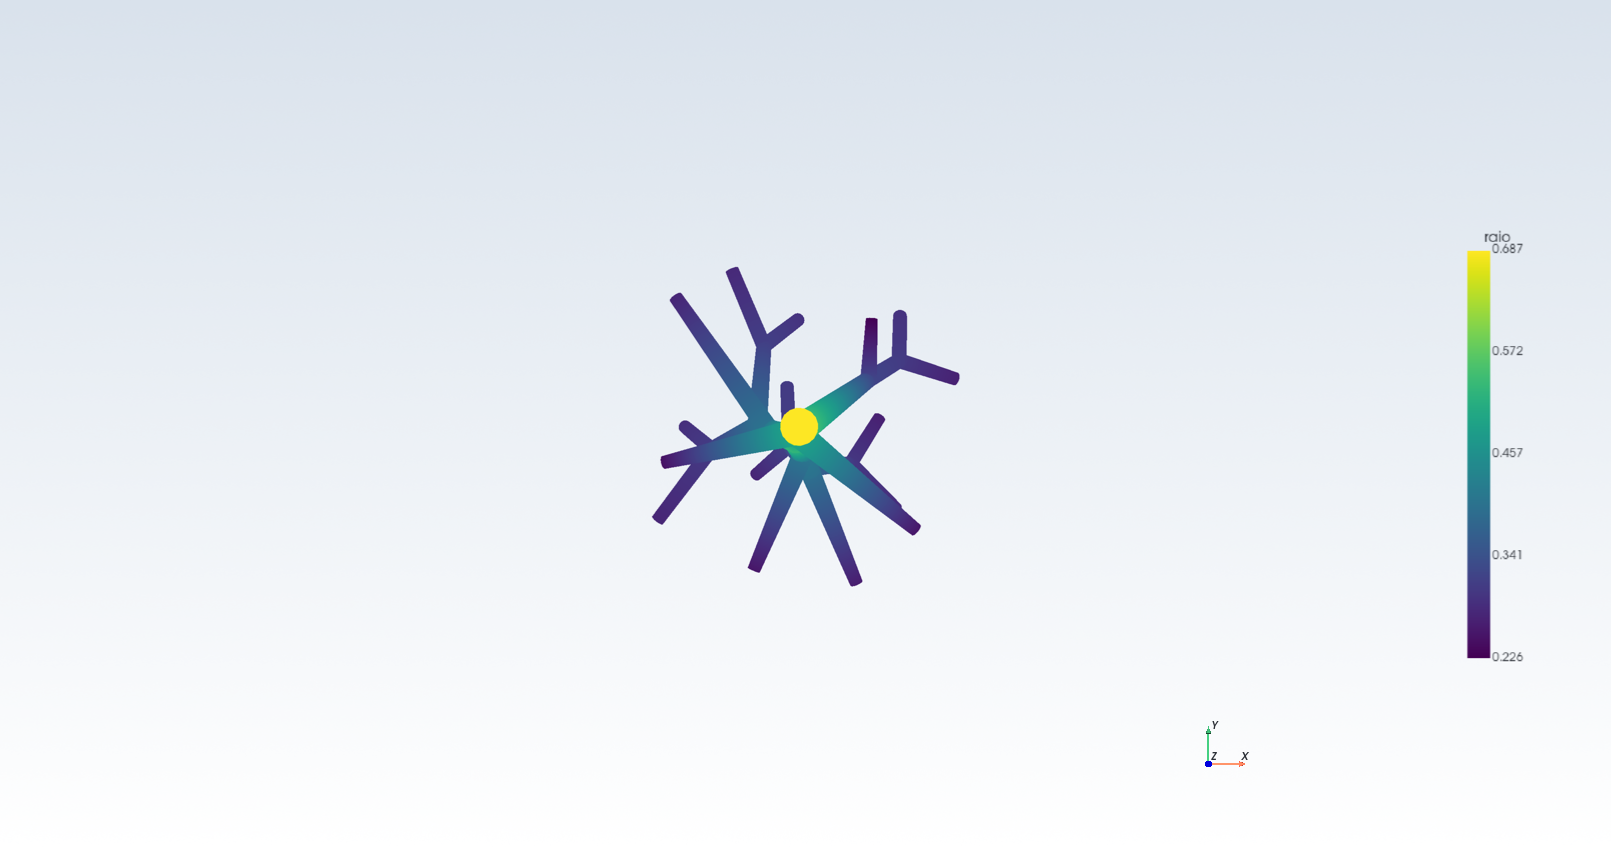
\includegraphics[width=0.24\linewidth]{figures/vista_frontal_persp.png}\hfill
 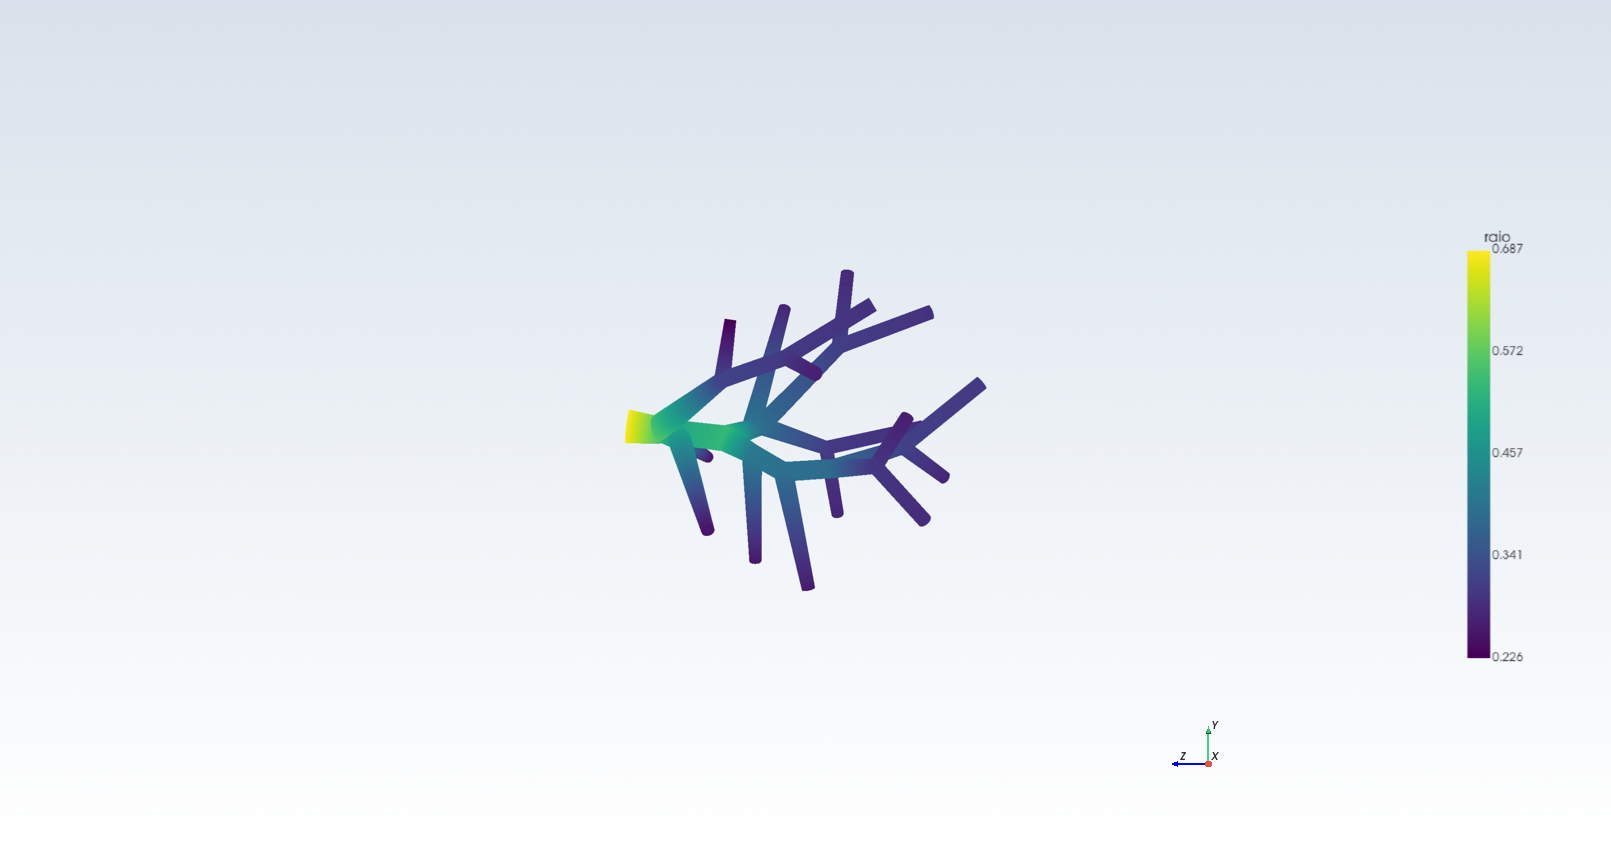
\includegraphics[width=0.24\linewidth]{figures/vista_lateral_persp.png}\hfill
 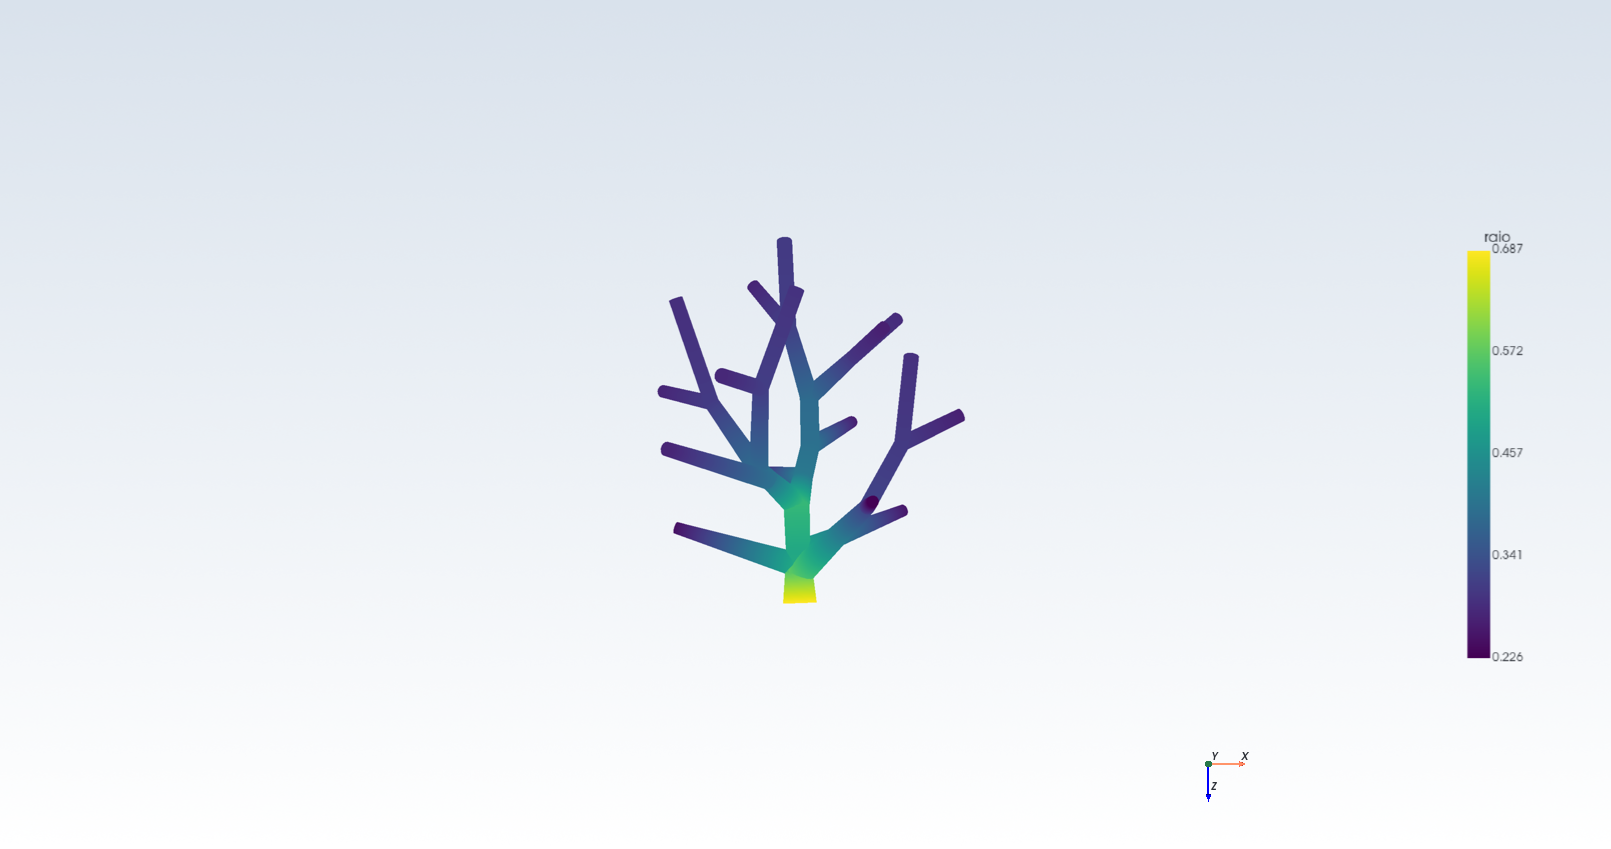
\includegraphics[width=0.24\linewidth]{figures/vista_topo_persp.png}\hfill
 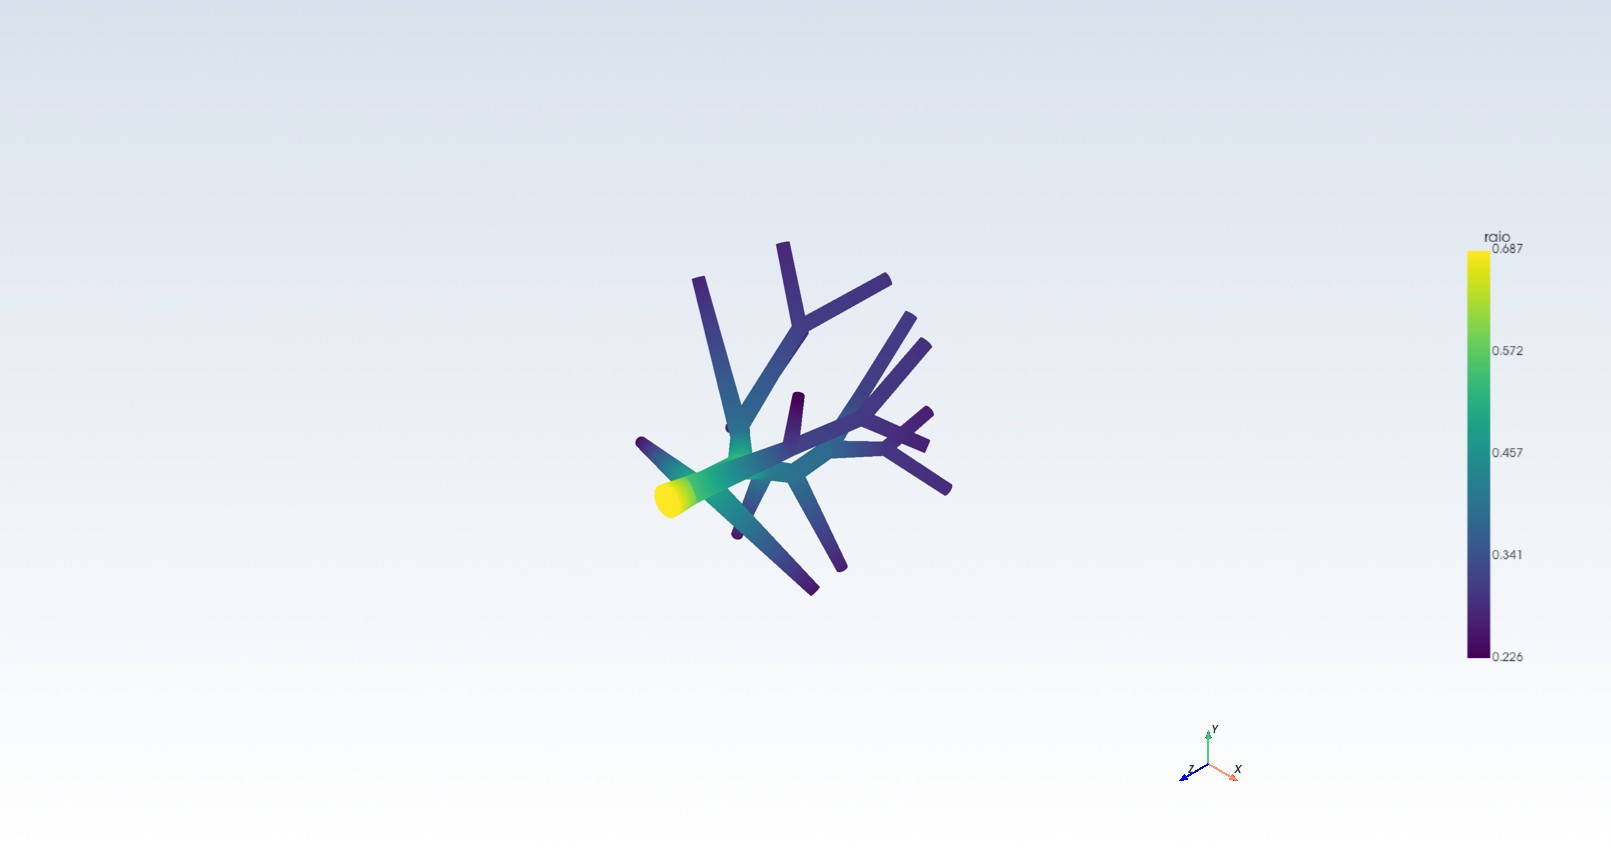
\includegraphics[width=0.24\linewidth]{figures/vista_isometrica_persp.png}}
 {\fbox{\parbox{0.8\linewidth}{\centering\color{red}\vspace{1.5em}
 Gerar com \texttt{visualizador.py ARQUIVO.vtk --exportar-vistas figures/}\vspace{1.5em}}}}
\caption{Quatro posições do observador (frontal, lateral, de topo e isométrica).}\label{fig:vistas}
\end{figure}

\figarq{projecoes}{0.95}{Projeção ortográfica (esq.) e perspectiva (dir.) da mesma árvore e da mesma vista.}{fig:proj}

Na ortográfica, vasos de mesmo comprimento aparecem com o mesmo tamanho,
independentemente da distância; na perspectiva, os mais distantes encolhem, o que dá
noção de profundidade, mas distorce comprimentos. Para modelos 2D (planos), as duas
projeções praticamente coincidem, e por isso a comparação só faz sentido nos modelos 3D.

\subsection{Módulo 3 -- Rasterização de linhas}
A Figura~\ref{fig:octantes} mostra o Bresenham nos oito octantes, com segmentos
partindo do centro de uma grade. Para o segmento $(2,1)\to(13,6)$, com $\Delta x=11$,
$\Delta y=-5$ e $e_0=6$, a Tabela~\ref{tab:bres} lista os 12 pixels, número igual a
$\max(|\Delta x|,|\Delta y|)+1$, e a Figura~\ref{fig:bresex} os mostra na grade.

\begin{table}[htbp]
\centering\small
\begin{tabular}{@{}rrrrrl@{}}
\toprule
$k$ & $x$ & $y$ & $e$ & $2e$ & próximo passo\\
\midrule
0 & 2 & 1 & 6 & 12 & $x$\\
1 & 3 & 1 & 1 & 2 & $x$ e $y$\\
2 & 4 & 2 & 7 & 14 & $x$\\
3 & 5 & 2 & 2 & 4 & $x$ e $y$\\
4 & 6 & 3 & 8 & 16 & $x$\\
5 & 7 & 3 & 3 & 6 & $x$ e $y$\\
6 & 8 & 4 & 9 & 18 & $x$\\
7 & 9 & 4 & 4 & 8 & $x$ e $y$\\
8 & 10 & 5 & 10 & 20 & $x$\\
9 & 11 & 5 & 5 & 10 & $x$ e $y$\\
10 & 12 & 6 & 11 & 22 & $x$\\
11 & 13 & 6 & 6 & 12 & fim\\
\bottomrule
\end{tabular}
\caption{Passo a passo do Bresenham para $(2,1)\to(13,6)$.}\label{tab:bres}
\end{table}

\fig{bresenham_octantes}{0.62}{Bresenham nos oito octantes (linha preta: segmento ideal).}{fig:octantes}
\fig{bresenham_exemplo}{0.8}{Pixels do exemplo numérico; o número indica a ordem de geração.}{fig:bresex}

Na validação, 1\,500 segmentos aleatórios (coordenadas em $[-30,30]$) satisfizeram:
extremos corretos, exatamente $\max(|\Delta x|,|\Delta y|)+1$ pixels, conectividade
em 8 vizinhos e desvio de no máximo $0{,}5$ pixel em relação à reta ideal. O DDA gerou um
conjunto de pixels diferente do Bresenham em 273 desses segmentos; em todos eles há pelo menos
um ponto em que a reta ideal passa exatamente a meio pixel, e os dois algoritmos desempatam de forma diferente.
Sobre a árvore projetada em 2D, o comando
\texttt{didatico.py bresenham --arvore ARQUIVO.vtk} rasteriza todos os segmentos
(Figura~\ref{fig:bresarv}) e informa quantos pixels diferem entre Bresenham e DDA.
No modelo \arq{tree2D\_Nterm008.vtk} (imagem $600\times600$, vista frontal), os 15
segmentos geram 1\,121 pixels em cada algoritmo, e 44 deles ficam em posições
diferentes: o programa imprime 88, que é o tamanho da diferença simétrica entre os
dois conjuntos (44 pixels só do Bresenham e 44 só do DDA).

\figarq{bresenham_arvore}{0.95}{Árvore rasterizada com o nosso Bresenham; à direita, zoom no segmento mais longo.}{fig:bresarv}

\subsection{Módulo 4 -- Rasterização de polígonos}
O polígono côncavo de teste, $[(2,1),(15,1),(15,11),(11,6),(7,11),(2,11)]$, tem um
entalhe em V, uma aresta horizontal e um vértice em que duas arestas começam na
mesma linha. A ET tem quatro arestas não horizontais
(Tabela~\ref{tab:et}); a varredura (Tabela~\ref{tab:aet}) mostra que, a partir de $y=6$,
a AET passa a ter quatro interseções e a linha ganha dois trechos.

\begin{table}[htbp]
\centering\small
\begin{tabular}{@{}rrrrr@{}}
\toprule
$y_{\min}$ & $y_{\max}$ & $x$ em $y_{\min}$ & $\Delta x$ & $\Delta y$\\
\midrule
1 & 11 & 2 & 0 & 10\\
1 & 11 & 15 & 0 & 10\\
6 & 11 & 11 & $-4$ & 5\\
6 & 11 & 11 & 4 & 5\\
\bottomrule
\end{tabular}
\caption{Tabela de arestas (ET) do polígono côncavo de teste.}\label{tab:et}
\end{table}

\begin{table}[htbp]
\centering\small
\begin{tabular}{@{}rll@{}}
\toprule
$y$ & interseções $x$ (AET ordenada) & trechos preenchidos\\
\midrule
1--5 & 2,00\quad 15,00 & [2, 14]\\
6 & 2,00\quad 11,00\quad 11,00\quad 15,00 & [2, 10] [11, 14]\\
7 & 2,00\quad 10,20\quad 11,80\quad 15,00 & [2, 10] [12, 14]\\
8 & 2,00\quad 9,40\quad 12,60\quad 15,00 & [2, 9] [13, 14]\\
9 & 2,00\quad 8,60\quad 13,40\quad 15,00 & [2, 8] [14, 14]\\
10 & 2,00\quad 7,80\quad 14,20\quad 15,00 & [2, 7]\\
\bottomrule
\end{tabular}
\caption{Varredura do \emph{Scanline Fill}: interseções e trechos por linha.}\label{tab:aet}
\end{table}

O preenchimento gera 114 pixels, para uma área geométrica de 110 (fórmula do
cadarço); a diferença vem da discretização: o contorno inclinado cobre pixels
parcialmente. Na validação, 300 polígonos estrelados aleatórios (em geral côncavos)
produziram exatamente os mesmos pixels que um teste independente de cruzamentos, que
não usa ET nem AET; dois quadrados vizinhos de $10\times10$ geraram 100 pixels cada,
sem sobreposição.

\fig{scanline_exemplo}{0.62}{\emph{Scanline Fill} no polígono côncavo (linha preta: contorno ideal).}{fig:scan}
\figarq{scanline_roi}{0.7}{Região de interesse (hexágono) preenchida sobre a árvore; o contorno usa o nosso Bresenham.}{fig:scanroi}

Sobre a árvore, o polígono é uma região de interesse hexagonal preenchida com
cor translúcida (Figura~\ref{fig:scanroi}), o que liga este módulo ao anterior.

\subsection{Módulo 5 -- Aliasing e antialiasing}
A comparação usa duas cenas. A primeira é um leque de retas a cada $15^\circ$
mais uma reta quase horizontal, que gera degraus longos e bem visíveis, em uma
imagem $64\times64$. A qualidade é medida pelo erro quadrático médio (EQM, escala
0--255) contra uma imagem de referência feita com supersampling de fator mais alto:
\begin{equation}
 \text{EQM}(A,B)=\frac{1}{3WH}\sum_{i,j,c}\bigl(A_{ijc}-B_{ijc}\bigr)^2 .
\end{equation}
Na cena de teste (referência $8\times8$), o EQM caiu de $2414{,}0$ (uma amostra por
pixel) para $54{,}1$ (SSAA $4\times4$), uma redução de cerca de 98\%. A imagem sem
antialiasing tem só 2 cores distintas (linha e fundo); com SSAA $4\times4$ passam a ser 17,
isto é, os 16 níveis de cobertura possíveis mais o fundo, que são os tons que
suavizam a escada (Figura~\ref{fig:aa}).

\fig{antialiasing_teste}{0.95}{Cena de teste sem antialiasing (esq.) e com supersampling $4\times4$ (dir.).}{fig:aa}
\figarq{antialiasing_arvore}{0.75}{Árvore sem e com SSAA, com zoom no segmento mais longo e EQM de cada caso.}{fig:aaarv}

Sobre a árvore (Figura~\ref{fig:aaarv}; modelo \arq{tree2D\_Nterm008.vtk}, imagem
$300\times300$), o programa informa os EQM contra a
referência (\texttt{--k 4 --ref 8}): sem AA, $49{,}06$; SSAA $4\times4$,
$3{,}95$; redução de 92\%. As cores distintas passam de 16 para 201. A comparação também pode ser vista na
janela 3D do visualizador: a tecla F2 liga e desliga o SSAA do VTK, que é a
técnica equivalente da biblioteca. Como a referência é, ela mesma, um
supersampling, o EQM mede a convergência para esse limite e não o erro em relação à
imagem ideal (ver Seção~\ref{sec:disc}).

\subsection{Módulo 6 -- Recorte de segmentos}
Os três algoritmos foram implementados e comparados; a janela é um retângulo e o
resultado de cada um é o trecho visível ou nada. No exemplo numérico, $P_0=(0,0)$,
$P_1=(12,10)$ e janela $x\in[2,10]$, $y\in[2,8]$, o Cohen--Sutherland precisa de duas
interseções (Tabela~\ref{tab:cs}) e o Liang--Barsky de quatro divisões, e ambos chegam
ao trecho $(2{,}40;\,2{,}00)\to(9{,}60;\,8{,}00)$ (Tabela~\ref{tab:lb}).

\begin{table}[htbp]
\centering\small
\begin{tabular}{@{}rlclcp{4.4cm}@{}}
\toprule
it & $P_0$ & $c_0$ & $P_1$ & $c_1$ & ação\\
\midrule
0 & (0,00;\,0,00) & 5 & (12,00;\,10,00) & 10 & $P_0$ vai para a borda base $\to$ (2,40;\,2,00)\\
1 & (2,40;\,2,00) & 0 & (12,00;\,10,00) & 10 & $P_1$ vai para a borda topo $\to$ (9,60;\,8,00)\\
2 & (2,40;\,2,00) & 0 & (9,60;\,8,00) & 0 & aceita\\
\bottomrule
\end{tabular}
\caption{Cohen--Sutherland no exemplo numérico (códigos: esq.=1, dir.=2, baixo=4, cima=8).}\label{tab:cs}
\end{table}

\begin{table}[htbp]
\centering\small
\begin{tabular}{@{}lrrrrrl@{}}
\toprule
borda & $p$ & $q$ & $r=q/p$ & $u_1$ & $u_2$ & ação\\
\midrule
esquerda & $-12$ & $-2$ & 0,1667 & 0,1667 & 1,0000 & entrada: $u_1=\max(u_1,r)$\\
direita & 12 & 10 & 0,8333 & 0,1667 & 0,8333 & saída: $u_2=\min(u_2,r)$\\
base & $-10$ & $-2$ & 0,2000 & 0,2000 & 0,8333 & entrada\\
topo & 10 & 8 & 0,8000 & 0,2000 & 0,8000 & saída\\
\bottomrule
\end{tabular}
\caption{Liang--Barsky no mesmo exemplo: $u_1=0{,}2$ e $u_2=0{,}8$.}\label{tab:lb}
\end{table}

A cena de teste tem dez segmentos e a janela $x\in[4,14]$, $y\in[3,9]$
(Figura~\ref{fig:rec}). Pelo Cohen--Sutherland, 1 foi aceito direto, 3 foram
rejeitados direto, 5 foram recortados e 1 foi rejeitado só depois de recortado:
o segmento $(2,8)\to(5,10{,}5)$ passa fora do canto superior esquerdo, e isso só se descobre
depois da primeira interseção. Os três algoritmos deram o mesmo resultado nos dez.

\fig{recorte_teste}{0.98}{Cena de teste antes (esq.) e depois (dir.) do recorte; a cor indica o caso do Cohen--Sutherland.}{fig:rec}
\figarq{recorte_arvore}{0.98}{Recorte da árvore: antes, depois (cinza: descartado) e rasterizado com Bresenham.}{fig:recarv}

Sobre a árvore (Figura~\ref{fig:recarv}; modelo \arq{tree2D\_Nterm008.vtk}, imagem
$300\times300$, janela $0{,}25$--$0{,}75$ da imagem, isto é, $x,y\in[75,225]$), o programa
conta os casos e as operações: 7 segmentos aceitos direto, 3 rejeitados direto,
5 recortados e nenhum rejeitado após recortar;
Cohen--Sutherland calculou 6 interseções e Liang--Barsky fez
57 divisões; os resultados são idênticos nos três algoritmos em
15 de 15 segmentos. Como 10 dos 15 segmentos se decidem só pelos códigos de região,
o Cohen--Sutherland faz bem menos contas aqui; o Liang--Barsky divide em quase
todas as bordas de todos os segmentos (57 de no máximo $15\times4=60$).

\paragraph{Os três algoritmos.} O Cohen--Sutherland é barato quando a maioria dos
segmentos se decide pelos códigos (aceitação ou rejeição trivial), mas pode calcular
interseções que depois se revelam inúteis, como no segmento~9. O Liang--Barsky usa
apenas comparações de $p$ e $q$ e faz no máximo uma divisão por borda, calculando
as interseções uma vez só, no final. O Cyrus--Beck faz o mesmo raciocínio
paramétrico, mas com normais e produtos escalares, o que o torna o único dos
três que serve para janelas convexas arbitrárias, ao custo de mais operações por borda.

\subsection{Módulo 7 -- Recorte de polígonos}
O Sutherland--Hodgman foi implementado para janela convexa qualquer (e não só
retangular) e testado em dois polígonos. O primeiro, convexo, tem vértices
$[(1,2),(9,0),(13,6),(8,11),(2,9)]$ e a janela é $x\in[3,11]$, $y\in[3,8]$. A
Tabela~\ref{tab:sh} mostra o resultado após cada borda; a área vai de 88 para 40.

\begin{table}[htbp]
\centering\small
\begin{tabular}{@{}lcp{9cm}@{}}
\toprule
\textbf{Borda} & \textbf{Vértices} & \textbf{Polígono resultante}\\
\midrule
base & 5 & (1,14;\,3) (11;\,3) (13;\,6) (8;\,11) (2;\,9)\\
direita & 5 & (1,14;\,3) (11;\,3) (11;\,8) (8;\,11) (2;\,9)\\
topo & 4 & (1,86;\,8) (1,14;\,3) (11;\,3) (11;\,8)\\
esquerda & 4 & (3;\,8) (3;\,3) (11;\,3) (11;\,8)\\
\bottomrule
\end{tabular}
\caption{Sutherland--Hodgman passo a passo no polígono convexo (uma borda por vez).}\label{tab:sh}
\end{table}

\fig{recorte_poligono_passos}{0.95}{Etapas do Sutherland--Hodgman e preenchimento do resultado com o nosso \emph{Scanline}.}{fig:shpassos}

O segundo polígono é côncavo, em forma de U, com vértices
\begin{center}\small
$(1,1),\,(17,1),\,(17,12),\,(12,12),\,(12,5),\,(6,5),\,(6,12),\,(1,12),$
\end{center}
recortado pela janela $x\in[2,16]$, $y\in[6,10]$. O resultado correto são \emph{dois} retângulos separados,
os dois braços do U, de área $16+16=32$. O algoritmo devolve, de fato, a área 32, mas como um único
polígono de 8 vértices, em que os dois retângulos são ligados por um trecho degenerado
de $(6,6)$ a $(12,6)$, percorrido nos dois sentidos (em vermelho na
Figura~\ref{fig:shu}). Quando o resultado só é desenhado com preenchimento, o defeito passa
despercebido, mas, ao desenhar o contorno ou ao usar o polígono em outras operações,
a aresta de largura zero aparece. Esse é o caso em que o Weiler--Atherton é o
algoritmo adequado, pois entregaria dois polígonos distintos.

\fig{recorte_poligono_concavo}{0.95}{Polígono em U e janela (esq.); resultado do Sutherland--Hodgman com a aresta degenerada em vermelho (dir.).}{fig:shu}
\figarq{recorte_poligono_arvore}{0.95}{Estrela côncava recortada sobre a árvore: antes (esq.) e depois (dir.), com Sutherland--Hodgman, \emph{Scanline} e Bresenham.}{fig:sharv}

Sobre a árvore (Figura~\ref{fig:sharv}), uma estrela de cinco pontas é recortada
e o resultado é preenchido com o \emph{Scanline} e contornado com o Bresenham do
grupo, integrando os módulos 3, 4 e 7.

\subsection{Autotestes}
Os módulos de rasterização e de recorte têm autotestes executáveis (\texttt{python src/rasterizacao.py}
e \texttt{python src/recorte.py}). Os resultados estão na Tabela~\ref{tab:testes}.

\begin{table}[htbp]
\centering\small
\begin{tabular}{@{}p{3.2cm}p{10.3cm}@{}}
\toprule
\textbf{Teste} & \textbf{Resultado}\\
\midrule
Bresenham & 1\,500 segmentos aleatórios: extremos, número de pixels, conectividade e desvio $\le0{,}5$ \\
\emph{Scanline} & 300 polígonos aleatórios iguais ao teste independente de cruzamentos; vizinhos sem sobreposição\\
Recorte de segmentos & 20\,000 pares segmento/janela: Cohen--Sutherland, Liang--Barsky e Cyrus--Beck coincidem; trechos dentro da janela e sobre a reta original\\
Sutherland--Hodgman & 600 polígonos (côncavos incluídos) $\times$ janelas aleatórias, 60 pontos cada: região resultante correta; quadrado $4\times4$ contra janela deslocada: área 4; janela disjunta: resultado vazio\\
\bottomrule
\end{tabular}
\caption{Resumo dos autotestes.}\label{tab:testes}
\end{table}

%% =====================================================================
\subsection{Discussão dos Achados}
\label{sec:disc}

\paragraph{Decisões de implementação.} Os módulos de matemática foram separados do VTK,
para que cada algoritmo possa ser lido, testado e demonstrado sem caixa-preta. O custo
é que a janela 3D interativa e a rasterização própria usam câmeras construídas por
caminhos diferentes: a primeira pelo VTK, a segunda pelas nossas matrizes. Para
reduzir essa diferença, a posição da câmera do VTK vem das nossas vistas e a ortográfica interativa usa
a mesma altura visível da perspectiva no plano do alvo.

\paragraph{Bresenham e DDA.} O Bresenham evita ponto flutuante e as divisões, e
produz os mesmos pixels em qualquer octante graças à forma simétrica. O DDA, mais simples,
difere em uma parte dos segmentos (273 de 1\,500 no teste), e em todos eles há pontos de empate (meio pixel).
Nenhum dos dois gera resultado visualmente errado; a preferência pelo Bresenham é
por precisão numérica e custo.

\paragraph{Antialiasing.} O SSAA suaviza a escada à custa de $k^2$ vezes mais
amostras (o tempo e a memória crescem com $k^2$). Como a referência do EQM é um
supersampling de fator $8$, a métrica mede a convergência para esse limite, não o erro em relação
à reta ideal; ainda assim, ela ordena corretamente as imagens. O filtro de caixa
é o mais simples e pode deixar bordas um pouco menos suaves que filtros maiores.

\paragraph{Recorte de segmentos.} Os três algoritmos concordaram em todos os casos testados,
exceto nos degenerados em que o segmento apenas toca um canto da janela, que o
autoteste ignora de propósito. Na prática, o Cohen--Sutherland é vantajoso quando a
maior parte dos segmentos está longe da janela, como no recorte de uma pequena região
da árvore; o Liang--Barsky é mais regular; e o Cyrus--Beck é a escolha quando a janela não é um
retângulo alinhado aos eixos.

\paragraph{Recorte de polígonos.} O Sutherland--Hodgman é simples e eficiente, mas
tem a limitação demonstrada na Figura~\ref{fig:shu}. O Weiler--Atherton resolve isso
e também aceita janelas côncavas; sua implementação completa não foi feita e
fica como possível extensão.

\paragraph{Limitações.} (i) A rasterização própria usa projeção ortográfica e
não resolve visibilidade (não há \emph{z-buffer}), assunto do TP2;
(ii) os vértices do \emph{Scanline} são inteiros, e por isso os polígonos vindos do
recorte (em ponto flutuante) são arredondados antes de preencher;
(iii) o recorte de segmentos e polígonos é 2D, em coordenadas de pixel;
(iv) o antialiasing do VTK (F2) é usado como está, sem controle do fator.

%% =====================================================================
\section{Conclusão}
O trabalho integrou, em uma aplicação única, os módulos pedidos: leitura e
visualização dos modelos CCO com cor por raio; transformações, vistas e as projeções ortográfica e
perspectiva; Bresenham, \emph{Scanline} e \emph{supersampling}; Cohen--Sutherland,
Liang--Barsky e Cyrus--Beck; e Sutherland--Hodgman. Os algoritmos foram escritos
a partir da matemática e conferidos por testes aleatórios, e o VTK foi usado para a leitura do arquivo, o desenho OpenGL, os tubos e,
na janela 3D interativa, a montagem das matrizes de vista e projeção a partir
das nossas câmeras; os algoritmos pedidos pelo enunciado são do grupo. O caso do
polígono em U mostrou na prática por que o Weiler--Atherton existe, e o código está
pronto para ser estendido com ele. Como próximos passos, o TP2 poderá usar a infraestrutura de
matrizes e rasterização para incorporar visibilidade, iluminação e técnicas baseadas
em raios.

%% =====================================================================

% --- AGRADECIMENTOS ---
\section*{Agradecimentos}
Os autores agradecem ao Departamento de Computação (DECOM) e à Universidade Federal de Ouro Preto (UFOP) pela infraestrutura e pelo suporte institucional, e ao Prof. Dr. Rafael Alves Bonfim de Queiroz pelos modelos CCO fornecidos e pelo enunciado do trabalho.

% --- REFERÊNCIAS BIBLIOGRÁFICAS ---
\begin{thebibliography}{99}
  \bibitem{schreiner1993} SCHREINER, W.; BUXBAUM, P. Computer-optimization of vascular trees. \textbf{IEEE Transactions on Biomedical Engineering}, v. 40, n. 5, p. 482--491, 1993.
  \bibitem{karch1999} KARCH, R.; NEUMANN, F.; NEUMANN, M.; SCHREINER, W. A three-dimensional model for arterial tree representation, generated by constrained constructive optimization. \textbf{Computers in Biology and Medicine}, v. 29, n. 1, p. 19--37, 1999.
  \bibitem{bresenham1965} BRESENHAM, J. E. Algorithm for computer control of a digital plotter. \textbf{IBM Systems Journal}, v. 4, n. 1, p. 25--30, 1965.
  \bibitem{sutherland1974} SUTHERLAND, I. E.; HODGMAN, G. W. Reentrant polygon clipping. \textbf{Communications of the ACM}, v. 17, n. 1, p. 32--42, 1974.
  \bibitem{weiler1977} WEILER, K.; ATHERTON, P. Hidden surface removal using polygon area sorting. \textbf{ACM SIGGRAPH Computer Graphics}, v. 11, n. 2, p. 214--222, 1977.
  \bibitem{liang1984} LIANG, Y.-D.; BARSKY, B. A. A new concept and method for line clipping. \textbf{ACM Transactions on Graphics}, v. 3, n. 1, p. 1--22, 1984.
  \bibitem{cyrus1978} CYRUS, M.; BECK, J. Generalized two- and three-dimensional clipping. \textbf{Computers \& Graphics}, v. 3, n. 1, p. 23--28, 1978.
  \bibitem{foley1990} FOLEY, J. D.; VAN DAM, A.; FEINER, S. K.; HUGHES, J. F. \textbf{Computer Graphics: Principles and Practice}. 2. ed. Reading: Addison-Wesley, 1990.
  \bibitem{vtk} SCHROEDER, W.; MARTIN, K.; LORENSEN, B. \textbf{The Visualization Toolkit}. 4. ed. Kitware, 2006.
  \bibitem{pyvista} SULLIVAN, C. B.; KASZYNSKI, A. A. PyVista: 3D plotting and mesh analysis through a streamlined interface for the Visualization Toolkit (VTK). \textbf{Journal of Open Source Software}, v. 4, n. 37, p. 1450, 2019.
  \bibitem{numpy} HARRIS, C. R. et al. Array programming with NumPy. \textbf{Nature}, v. 585, p. 357--362, 2020.
  \bibitem{matplotlib} HUNTER, J. D. Matplotlib: a 2D graphics environment. \textbf{Computing in Science \& Engineering}, v. 9, n. 3, p. 90--95, 2007.
\end{thebibliography}

\end{document}